% !TeX root = ../main.tex

\chapter{A Fully-Convolutional LSTM Encoder-Predictor Model} \label{chapter:implementation}

This chapter presents the final model that is used in this thesis for future frame prediction. It combines the insights and strengths of previous works that have been analyzed in the previous chapter. Each component of it is investigeted in detail and then assembled to end up with the overall network architecture. But beforehand, two cruical techniques are presented that improved learning spatio-temporal featues and recurrent training performance.

\section{Techniques}

In this section, two important methods are presented that enable recurrent network based models to reach better performance in a shorter training time. These techniques are then used as building blocks in the description of the network architecture.

\subsection{Convolutional LSTM} \label{sec:conv_lstm}

As discussed in earlier chapters, the standard LSTM cell has the drawback of lacking spatial correlations in the input-to-hidden and hidden-to-hidden transitions, because it operates over sequences of vectors with only one dimension. The LSTM activations are computed based on linear transformations using fully-connected layers and subsequent non-linearities. The authors of \parencite{conv_lstm_nowcasting} proposed a variant of the LSTM cell with the core idea to handle all inputs, hidden states, cell or gate outputs are 3D tensors to preserve spatial properties of the data. This is realized by enchanging the matrix products by the convolution operation. The resulting recurrent cell is called \textit{convolutional LSTM} (ConvLSTM).

In contrast to the realization in \parencite{spat_temp_video_autoenc}, peephole connections are included in our ConvLSTM implementation. These allow the gates to have an direct access to the previous memeory cell state. In addition, we enable it to use optional batch normalization layers in both input-to-hidden and hidden-to-hidden transitions as proposed in \parencite{rnn-batchnorm} to allow faster learning and take advantage of other benefits that have been described in section \ref{sec:batch_norm}. All this together can be formulated as:

%TODO maybe correct this formula, since we used conv2d instad of hadamard for peepholes as well.
\begin{equation} \label{eq:convlstm}
\begin{aligned}
\Spvek{\tilde{\textbf{f}}^{(\tau)}; \tilde{\textbf{i}}^{(\tau)}; \tilde{\textbf{o}}^{(\tau)}} &= \texttt{BN}(\textbf{W}_{h} \ast \textbf{h}^{(\tau-1)}; \gamma_h, \beta_h) + \texttt{BN}(\textbf{W}_{x} \ast \textbf{x}^{(\tau)}; \gamma_x, \beta_x) + \textbf{W}_{peep} \odot \textbf{C}^{(\tau-1)} + \textbf{b} \\
\hat{\textbf{c}}^{(\tau)} &= tanh(\texttt{BN}(\textbf{W}_{hc} \ast \textbf{h}^{(\tau-1)}; \gamma_h, \beta_h) + \texttt{BN}(\textbf{W}_{xc} \ast \textbf{x}^{(\tau)}; \gamma_x, \beta_x) + \textbf{b}_c) \\
\textbf{C}^{(\tau)} &= \sigma(\tilde{\textbf{f}}^{(\tau)}) \odot \textbf{C}^{(\tau-1)} + \sigma(\tilde{\textbf{i}}^{(\tau)}) \odot \hat{\textbf{c}}^{(\tau)} \\
\textbf{h}^{(\tau)} &= \sigma(\tilde{\textbf{o}}^{(\tau)}) \odot tanh(\texttt{BN}(\textbf{C}^{(\tau)}; \gamma_c, \beta_c))
\end{aligned}
\end{equation}

where $ \textbf{W}_h \in \mathbb{R}^{d_h \times 3d_h} $ and $ \textbf{W}_{hc} \in \mathbb{R}^{d_h \times d_h} $ are the shared weights for the hidden to hidden transitions at time step $ \tau $, $ \textbf{W}_x \in \mathbb{R}^{d_x \times 3d_h} $ and $ \textbf{W}_{xc} \in \mathbb{R}^{d_x \times d_h} $ the shared weights for the input to hidden connections, $ \textbf{W}_{peep} \in \mathbb{R}^{d_x \times 3d_h} $ the shared weights for the peephole connections, $ \textbf{b} \in \mathbb{R}^{3d_h} $ and $ \textbf{b}_c \in \mathbb{R}^{d_h} $ the biases, and $ \textbf{C}^{(0)}, \textbf{h}^{(0)} \in \mathbb{R}^{4d_h} $ the initial states of the memory cell and the hidden state, respectively. Further, $\ast$ denotes the convolution operation and $ \texttt{BN}(\textbf{x}; \gamma, \beta) $ a batch normalization layer with learned shift $\gamma$ and scale $\beta$. As in \parencite{rnn-batchnorm}, $\beta_h$ and $\beta_x$ are set to zero by default to avoid the unnecessary redundancy with the existing bias terms $\textbf{b}$ and $\textbf{b}_c$. The structure of such a cell in visualized in Figure \ref{fig:convlstm-cell}.

\begin{figure}[htpb]
	\centering
	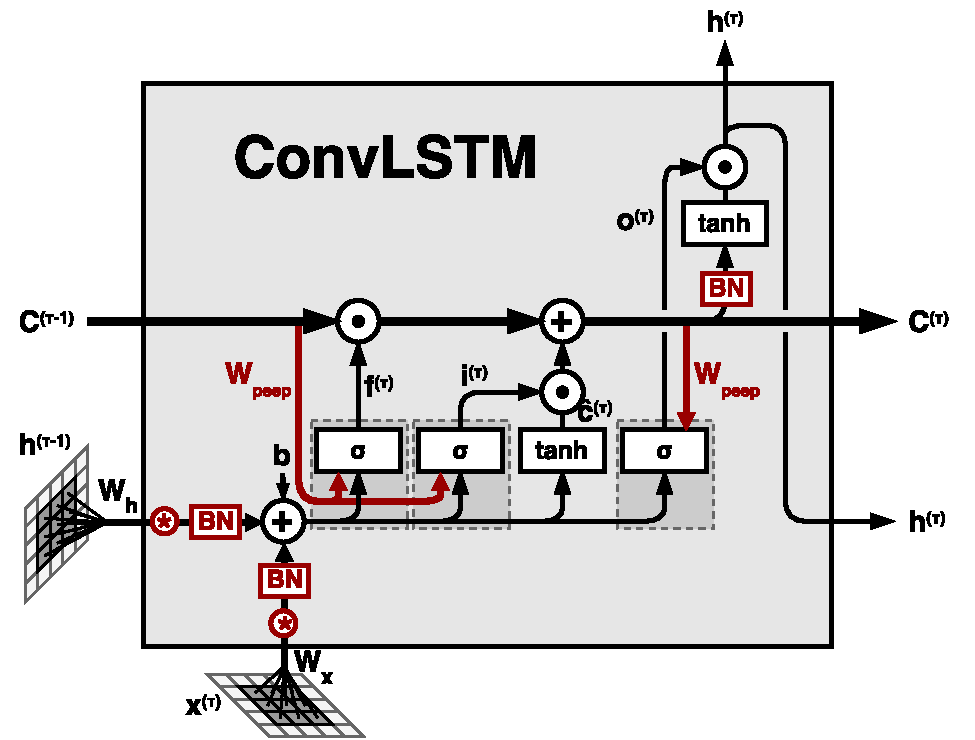
\includegraphics[width=0.7\linewidth]{figures/convlstm.pdf} 
	\caption[ConvLSTM Cell]{The simplified structure of the batch-normalized ConvLSTM cell. The inputs and previous hidden states are convolved and produce 3D tensors that flow through each cell. Changes to standard FC-LSTM are in red.} \label{fig:convlstm-cell}
\end{figure}


\subsection{Scheduled Sampling} \label{sec:sched_sample}

%recurrent training strategy (has not been used in context of frame prediction so far)
%Explain schedules sampling and the problem why it is needed. Compare it agains "Always sampling".
% ==> learns a robustness.

When the first recurrent network based models have been tested in the course of this thesis, a discrepancy between training and inferance has been discovered. At training, each cell is usually fed with the ground truth $\textbf{x}^{(\tau-1)}$ of the previous time step in order to generate the current prediction $\hat{\textbf{x}}^{(\tau)}$. In contrast, the generated frame $ \hat{\textbf{x}}^{(\tau-1)}$ of the previous cell is used instead as cell input during inference, because no ground truth is available in that case. Thus, mistakes made early in the sequence flow through all following cells and can quickly amplify since the network has never dealt with such errors at training time. In context of future frame generation, this effect has been identified when the prediction quality starting from second frame has dropped tremendously. The fact that generated frames usually look slightly blurry is the clear reason for this, because a network that was fed with ground truth input images only has never seen such pictures.

As a first step, the recurrent cell input during the training process has therefore been adapted to behave in the same way as in inference mode. Therefore, a recurrent cell that is trained to generate a future frame has to condition on the previously generated frame instead the ground truth. Using such a strategy, the model learns to be more robust. However, this comes with the downside that the RNN model converges much slower during the training, because it has to predict the correct output given an imperfect or even wrong input.

To combine the best of both worlds, we experimented with a training strategy where each recurrent cell started to condition on the ground truth frame and slowly changed to the inference mode conditioning using a probability variable $p$ with linear of exponential decay. Therefore, a random number $r \in [0, 1]$ is generated at each training step and we condition on the generated frame when $r \geq p$. First results have shown positive results where a better performance could be reached compared both other strategies mentioned earlier. 

Shortly afterwards, we came across \parencite{sched_sample} where the authors propose a similar but even more radical strategy and demonstrate insightful evaluation results. Their so-called \textit{scheduled sampling} training strategy for recurrent networks is based on the same core idea, but instead of generateing a random number $r$ for a whole input sequence only, they propose to do this for every single time step $\tau$. In addition, they suggest to use an inverse sigmoid decay function in order to provide a smooth transition from training mode to inference mode:

\begin{equation} \label{eq:inverse-sigmoid}
\sigma_{inv}(i; \alpha) = \frac{\alpha}{\alpha + exp(i / \alpha)} ,
\end{equation}

where $i$ indentifies the current training step and $\alpha \geq 1$ controls the expected speed of convergence. This function, as well as a diagram of the scheduled sampling approach is depicted in Figure \ref{fig:sched-sample}.

%TODO Figure a) inverse sigmoid b) scheduled sampling mock
\begin{figure}[htpb]
\centering
\begin{subfigure}{0.5\textwidth}
  \centering
  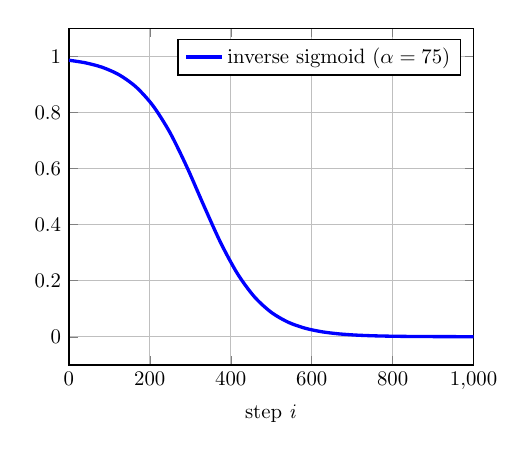
\begin{tikzpicture}[scale=0.75]
    \begin{axis}[
        ymin=-0.1,
        ymax=1.1,
        xmin=0,
        xmax=1000,
        legend style={legend pos=north east},
        grid,
        thick,
        xlabel=step \textit{i},
      ]
      \addplot [mark=none,draw=blue,smooth,ultra thick,domain=0:1000] {75/(75+exp(\x / 75))};
      \addlegendentry{inverse sigmoid ($\alpha = 75$)};
    \end{axis}
  \end{tikzpicture}
  \caption{}
  \label{fig:sched-sample-inv-sig}
\end{subfigure}%
\begin{subfigure}{0.5\textwidth}
  \centering
  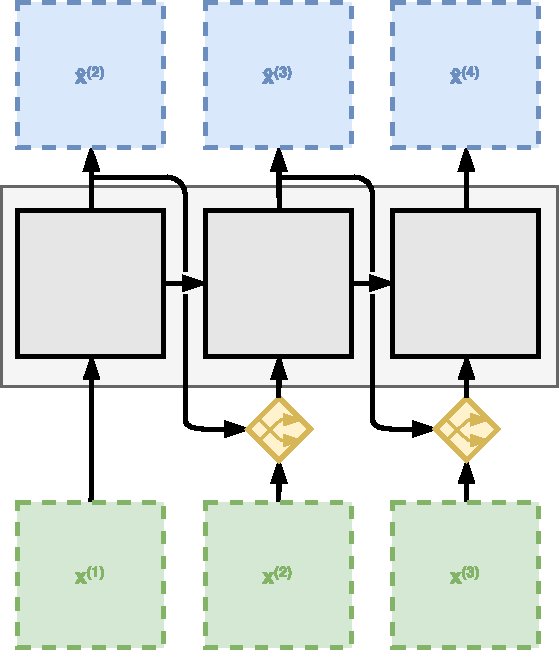
\includegraphics[width=.8\linewidth]{figures/sched_sample.pdf}
  \caption{}
  \label{fig:sched-sample-process}
\end{subfigure}
\caption[Scheduled Sampling]{Illustrations of scheduled sampling, where (a) shows the inverse sigmoid function and (b) the structure of a RNN that uses this approach. The yellow block symbolize the scheduled sampling components, which decide whether the cell conditions ont the ground truth or the previous output by flipping an unbiased coin.} \label{fig:sched-sample}
\end{figure}




\section{Network Architecture}

The final model architecture is based on the RNN encoder-decoder model introduced in Section \ref{sec:rnn_enc_dec}, both previously presented techniques and advancements to improve the learning of both spatial and temporal features in video data. This architecture has been chosen because it explicitely models the temporal correlations and is flexible regarding the input and output sequence. Further, previous works demonstrated in Chapter \ref{chapter:relatedwork} have shown promising results using this recurrent framework. The architecture that is presented in this section describes the vanilla version of the network that is used for frame prediction of Moving MNIST sequences. The following evaluation in Chapter \ref{chapter:evaluation} assesses the model with different settings, such as variations in depth.

\subsection{Components}

Before the entire network model is demonstrated, we would like to go through its four main components in detail first. These components for encoding or decoding are ordered according to the flow of data while inference.

\subsubsection{Spatial Encoder}

Instead of feeding the recurrent encoder with raw image data directly like in \parencite{unsup_learn_lstm} or \parencite{conv_lstm_nowcasting}, each frame flows through a multilayer CNN first in order to project it to an image percept in feature space of lower height and witdth, but higher depth. This single convolutional network is shared accross the entire time domain of the following spatio-temporal encoder network. The motivation for this spatial encoder is based on \parencite{spat_temp_video_autoenc} who suggested that a deeper encoding of the input image could yield better results. Furthermore, decreasing the height and width of the image has a very positive impact on the overall runtime and memory efficient. And even when the total dimensionality of convolved frame percepts is higher than the original image due to the higher number of feature maps, it does not harm these two advantages in overall model efficiency, because the ConvLSTM cells in the recurrent encoder increase to percept's depth either way. The spatial encoder component is illustrated in Figure \ref{fig:comp-spatial_encoder}.

\begin{figure}[htb]
	\centering
	
\includegraphics[width=0.6\linewidth]{figures/placeholder.png} 
	\caption[Spatial Encoder Component]{tbd} \label{fig:comp-spatial_encoder}
\end{figure}

No max pooling layers have been used because rotation tolerance would be counter-productive in context of frame prediction. This kind of downsampling could also remove important details that might be required to successfully reconstruct the image. Instead, each frame is downsampled by using a stride of $ s=2 $ in specific convolutioal layers with the motivation that the network itself learns how to perform such a downsampling operation. Additionally, each convolutional layer is activated using ReLUs and followed by a batch normalization layer to compensate the internal covariate shift of such a deep network model. The resulting frame percepts exhibit a shape of $16\times16\times64$.

\subsubsection{Spatio-Temporal Encoder}

The percept tensors that have been produced by the spatial encoder CNN for each frame of the sequence then flows into a recurrent network to preserve sequential correlations and to learn temporal dynamics. To be more precise, ConvLSTM cells are used that retain the spatial strutucture of the three-dimensional input data. The cell state $C^{(0)}$ and hidden state $h^{(0)}$ of the spatio-temporal encoder network are initialized with zero by default. Moreover, all convolutions within the ConvLSTM cells produce the adapt number of produced feaures maps according to the input's depth in order to keep all shape sizes constant. After the whole input sequence of about ten frames has been processed, the resulting cell and hidden states then ecode the learned representation of motion within the sequence. This representation is then transfered to the next prediction component. It should be noted that the hidden outputs of the encoder's ConvLSTM cells are discared and not used in the subsequent decoding network. The spatio-temporal encoder component is shown in Figure \ref{fig:comp-spatiotemp_encoder}.

\begin{figure}[htb]
	\centering
	
\includegraphics[width=0.6\linewidth]{figures/placeholder.png} 
	\caption[Spatio-Temporal Encoding Component]{tbd} \label{fig:comp-spatiotemp_encoder}
\end{figure}

\subsubsection{Spatio-Temporal Predictor}

Initialized by the cell and hidden state of the previous ConvLSTM encoder, the recurrent predictor component takes over to map each frame in feature space at time step $\tau$ to its future representation at time step $\tau + 1$. The spatio-temporal decoder takes advantage of the ConvLSTM cells one more, but it handles the inputs and outputs to each cell in a different way.

\begin{figure}[htb]
	\centering
	
\includegraphics[width=0.6\linewidth]{figures/placeholder.png} 
	\caption[Spatio-Temporal Predictor Component]{tbd} \label{fig:comp-spatiotemp_predictor}
\end{figure}

As depicted in Figure \ref{fig:comp-spatiotemp_predictor}, the prediction component utilizes the schedules sampling technique earlier presented in Section \ref{sec:sched_sample} to improve the training performance. By default, the network begins to condition on percepts in feature space of the ground truth frame produced by the spatial encoder component. By decaying the probability of conditioning on the ground truth using an inverse sigmoid function with $\alpha = 1000$, the predictor RNN slowly starts to condition of the previously generated frames as in inference mode. With this setting, it takes about \num{10000} training steps until this component generates future frame representations entirely based on previous outputs. After the entire output sequence has been generated, each single tensor still exhibit a shape of size $16\times16\times64$ and altogether represent the video's future in feature space.

\subsubsection{Spatial Decoder}

To map each frame representation back to the original image space, a second CNN is modelled that performs the same transformation steps of the spatial encoder in reverse order. It therefore uses transposed convolution layers with rectifier units and batch normalization layers in-between. However, the activation function of the output layer is either a sigmoid or a hyperbolic tangent function to ensure that the generated frames exhibit a valid scale of values. The described spatial decoder is illustrated in Figure \ref{fig:comp-spatial_decoder}.

\begin{figure}[htb]
	\centering
	
\includegraphics[width=0.6\linewidth]{figures/placeholder.png} 
	\caption[Spatial Decoder Component]{tbd} \label{fig:comp-spatial_decoder}
\end{figure}


\subsection{Model}

To see everything at a glance, each previously described component is put together in Figure \ref{fig:total_model} to demonstrate the entire model. Since the overall architecture follows the concept of an encoder-decoder network, it should be argued why this model is likely to learn useful features. According to the argumentation in \parencite[p. 3f.]{unsup_learn_lstm}, it is unlikely to learn the trivial function for the following two reasons. First, an entire sequence of variable size and the temporal dynamics have to be encoded and decoded using a fixed-sized representation. In order accurately predict future frames multiple frames ahead, the decoder network really has to come up with a learned representation that can distinguish several foreground objects from static background, as well as understand the motion of object and the environmental constraints within a given video scene.

\begin{figure}[p]
	\centering
	
\includegraphics[width=0.8\linewidth]{figures/placeholder.png} 
	\caption[LSTM Encoder-Predictor Model]{tbd} \label{fig:total_model}
\end{figure}

% here: add loss - layer as well! (red box?)
% mention that weights are shared when the components have the same color? Or make dotted boxes? Or say layer-wise shared?


















%\subsection{Loss function} ??? / Loss-layer
